\chapter{Theoretical Foundations}
\label{ch_introduction}

\begin{chapterinfo}
    This chapter is a general introduction to accelerator physics.
    The goal of this introduction is to collect all the necessary tools that are needed to develop
    the methods and algorithms presented in the main part of this thesis.
    Therefore we need a sound understanding of linear beam optics, 
    $\beta$~function, phase and coupling.
    Only a brief summary of the vast field of accelerator physics can be given in the scope of this
    thesis. The interested reader may consult some of the great introductory works of the field, e.g.
    \cite{CAS2003, Wiedemann2015, WolskiBook}.

    Also the normal form approach shall be introduced here as it is needed to calculate optics
    parameters from Hamiltonian terms in chapter~\ref{ch_localobs}.

\end{chapterinfo}

%\section{A word on notation}
%Accelerator physics is a field, for sure not the only one, with notoriously bad notation and conventions.
%In multiple cases the same symbol is used to describe two or more completely different quantities.
%Keeping the notation of a work like this PhD thesis consistent is not an easy task on its own. Less so
%in the given situation.
%Therefore this little prolog serves in guiding the reader through the notations and conventions adopted
%throughout this thesis.
%\textbf{Planes} We describe the motion of the particles and beams in the regime of \emph{transverse beam dynamics} with
%two transverse planes $x$ and $y$.
%So we have to distinguish optical functions and variables by plane: $x, y, \beta_x, \alpha_x, \phi_x$.
%Most of the time however it is of no importance in which plane the equations
%are expressed or we work for an extended period in the same plane.
%In those cases, the index denoting the plane will be dropped. 
%\textbf{Vectors} are denoted by an italic letter with an arrow above. Phase space \textbf{coordinates} are
%usually denoted by lowercase latin letters ($\vec{x}, \vec{v}, \vec{p}$) with the exception of normal form coordinates
%which are greek lowarcase letters ($\vec{\zeta}, \vec{\xi}$). \textbf{Fields} are denoted by capital
%latin letters ($\vec{E}, \vec{B}$).
%\textbf{Matrices} are denoted by bold face letters, usually capital latin $\mat{M}, \mat{V}$.




%The Large Hadron Collider is the world's largest particle accelerator with the highest center of mass
%energy per charge unit. It has a circumference of $\SI{27}{km}$ and is situated at the French-Swiss 
%border near Geneva. The top energy for protons is $\SI{7}{TeV}$
%and in the lead ion run of 2018 a beam energy of $\SI{6.37}{Z TeV}$ was achieved.
%The particles pass through various pre-accelerators where they are accelerated in steps before being
%injected in the LHC at $\SI{450}{GeV}$. The complete accelerator complex at CERN is sketched in
%\figref{fig_cern_acc_cmplx}.

% --------------------------------------------------------------------------------------------------
% beam optics
% --------------------------------------------------------------------------------------------------
\section{Beam Optics}

Very much like light beams, charged particle beams in an accelerator can be bent, focused, defocused
and can be subject to effects like dispersion and chromaticity. Therefore the term \emph{optics} is
generally used to describe the movement and behaviour of particle beams around the accelerator.

This work focuses on single particle dynamics, effects between the particles of a beam will be
neglected. 

\subsection{Linear Beam Dynamics}

Linear beam dynamics studies the effect of linear electromagnetic fields on the particles.
This includes primarily only drift spaces, bending magnets and (de)focusing magnets. Under the presence
of electromagnetic fields $\vec{E}$ and $\vec{B}$, the Lorentz force acts on the particles with charge
$q$ and velocity $\vec{v}$.
%
\begin{equation}
    \vec{F} = q\left(\vec{E} + \vec{v} \times \vec{B}\right)
    \fstop
    \label{eq_lorentz_force}
\end{equation}
%
A dipole with a constant magnetic field $B_y$ bends a particle's trajectory into an arc of radius $\rho$
%
\begin{equation}
    \rho = \frac{p}{qB_y}
    \fstop
    \label{eq_acc_radius}
\end{equation}
%
It is useful to describe the motion in a circular accelerator in a co-moving reference frame as
depictet in \figref{fig_frenet_serret}\index{Frenet-Serret coordinates} where the cartesian coordinates $\{x', y', z'\}$ are
transformed into a system $\{x,y,s\}$ with the properties:
%
\begin{align}
    \Delta s &\parallel \text{reference orbit}\notag\\
    \hat{y} &= \hat{y}'\notag\\
    \hat{x} &= \hat{y} \times \Delta s
\end{align}
%
and a longitudinal coordinate $s$ along the reference orbit.
\begin{figure}[h]
    \includestandalone{frenetserret}
    \caption{
        The Frenet-Serret coordinate system which is moving along the design orbit of particles
        in the accelerator.
    }
    \label{fig_frenet_serret}
\end{figure}
%
As reference orbit the so called closed orbit is normally used. The properties of the closed orbit
will be explained in a moment.

In this coordinate system the motion of a particle in a circular accelerator is described by Hill's
differential equation\index{Hill's equation}:
%
\begin{equation}
    \frac{\der^2 z}{\der s^2} + k(s)z = 0
    %\fstop
    \label{eq_hills}
\end{equation}
%
where $z \in \{x,y\}$ is the transverse coordinate and $k(s)$ is the linear magnet strength at
position $s$.

A solution that satisfies \eqref{eq_hills} is
%
\begin{equation}
    z(s) = A_z(s) \cos\left(\phi_z(s) + \phi_{z,0} \right)
    \label{eq_betatron_osc}
\end{equation}
%
where the $s$-dependent amplitude of the oscillation can be split:
%
\begin{equation}
    A_z(s) = \sqrt{2J_z \beta_z(s)}
    \fstop
    \label{eq_betatron_ampl}
\end{equation}
%
$\beta_z(s)$ is the $s$-dependent part of the amplitude, called $\beta$~function\index{$\beta$ function}.
$J_z$ is the action invariant of the particle's motion.
$\beta(s)$ and $\phi(s)$\index{betatron phase}\index{phase} are periodic with the circumference of the ring $C$.

Of special interest for a collider is the value of the $\beta$~function at the interaction point,
denoted as $\beta^* \equiv \beta(s_\text{IP})$ because it defines the beam size and
has a high impact on the luminosity, as follows from \eqref{eq_lumi}.

$\phi(s)$ is called the \emph{betatron phase} and satisfies the following property:
%
\begin{equation}
    \phi(s_1) - \phi(s_0) = \int\limits_{s_0}^{s_1} \frac{1}{\beta(s)}\der s
    \fstop
    \label{eq_phase}
\end{equation}
%
The trajectories of particles with an action $J$ are limited by an envelope function $\sqrt{2J\beta}$ as illustrated in Fig.~\ref{fig_part_traj}.
%
\begin{figure}[h]
    \centering
    \includestandalone[width=.49\linewidth]{particle_traj_beta_1}
    \hfill
    \includestandalone[width=.49\linewidth]{particle_traj_beta_many_wb} 
    \caption{The trajectories of particles with action $J$ are shown.}
    \label{fig_part_traj}
\end{figure}
%
Actual $\beta$~functions are shown in Fig.~\ref{fig_beta}.
%
\begin{figure}[h]
  \centering
  \footnotesize
  \includestandalone[width=\linewidth]{./twiss/IP_beta_x}
  \includestandalone[width=\linewidth]{./twiss/Arc_beta_x}
  \normalsize
  \caption{
    TOP: The $\beta$~function around IP1.
    BOTTOM: The $\beta$~functions in an LHC arc, the plot ranges from IP to IP.
    Both plots show the LHC collision optics at $\beta^*=\SI{30}{cm}$.
  }
  \label{fig_beta}
\end{figure}

Solutions of \eqref{eq_hills} for linear lattice elements can be expressed in matrix form
%
\begin{equation}
    \begin{pmatrix}
        z_b\\
        z_b'
    \end{pmatrix}
    =
    \begin{pmatrix}
        m_{11} & m_{12} \\
        m_{21} & m_{22}
    \end{pmatrix}
    \begin{pmatrix}
        z_a\\
        z_a'
    \end{pmatrix}
    \fstop
    \label{eq_matrix_element}
\end{equation}
%
The matrix 
%
\begin{equation}
    \mat{M} = 
    \begin{pmatrix}
        m_{11} & m_{12} \\
        m_{21} & m_{22}
    \end{pmatrix}
    \label{eq_trmat}
\end{equation}
%
is called the \emph{transfer matrix}\index{transfer matrix}. It describes the transformation
of phase space when going from one position $s_a$ in the lattice to another $s_b$.

For illustration the transfer matrix of a focusing quadrupole will be given.
For $s$ inside the magnet $k(s) = k_1$ . The solution of Hill's equation is
%
\begin{equation}
    z(s) = \cos \left[ \sqrt{k}(s-s_0)\right] z_0 + \frac{1}{\sqrt{k}}\sin\left[\sqrt{k}(s-s_0)\right]z_0'
    \fstop
\end{equation}
%
The transfer matrix of a focusing quadrupole reads
%
\begin{equation}
    \mat{M}_{QF} =
    \begin{pmatrix}
        \cos \sqrt{K} & \frac{1}{\sqrt{k}} \sin \sqrt{K} \\
        -\sqrt{k}\sin \sqrt{K} & \cos \sqrt{K}
    \end{pmatrix}
\end{equation}
%
where $K$ is the integrated magnet strength
%
\begin{equation}
    K = \int\limits_{s_i}^{s_i + L} k(s)\der s
\end{equation}
%
for a quadrupole at position $s_i$ with length $L$.

A purely linear accelerator can than be constructed by the composition of the transfer matrices of 
all its elements. This composition yields a special example of the transfer matrix, the one that
transforms the phase space coordinates of a particle at a given position to the same position in the
next turn\index{one turn map}:
%
\begin{equation}
    \mat{M}_\text{OT} = \prod\limits_{w=0}^W \mat{M}_i
\end{equation}
%
where $\mat{M}_w$ is the transfer matrix of the $w$th element, $W$ is the number of elements in the
accelerator and the product denotes the repeated matrix multiplication from the left.

The phase advance of one turn
%
\begin{equation}
    Q_z \equiv \frac{1}{2\pi}\int\limits_{s_0}^{s_0+C} \frac{\der s}{\beta_z(s)}
    \komma
\end{equation}
%
normalised by $2\pi$, is called the \emph{betatron tune}\index{tune}\index{betatron tune}.

A general form of \eqref{eq_trmat} is 
%
\begin{equation}
    \begin{pmatrix}
        \sqrt{\frac{\beta_b}{\beta_a}}(\cos\phi_{ab} + \alpha_a \sin\phi_{ab}) &
        \sqrt{\beta_a\beta_b} \sin\phi_{ab} \\
        \frac{\alpha_a - \alpha_b}{\sqrt{\beta_a\beta_b}}\cos\phi_{ab} - \frac{\beta+\alpha_a\alpha_b}{\sqrt{\beta_a\beta_b}}\sin\phi_{ab} &
        \sqrt{\frac{\beta_a}{\beta_b}}(\cos\phi_{ab} - \alpha_b\sin\phi_{ab})
    \end{pmatrix}
    \label{eq_trmat_01}
\end{equation}
%
where the quantity
%
\begin{equation}
    \alpha(s) = -\frac{1}{2}\frac{\der \beta(s)}{ \der s}
    \label{eq_alpha}
\end{equation}
%
is called $\alpha$~\emph{function}\index{$\alpha$ function}.
%
$\alpha$, $\beta$ function and a third quantity
%
\begin{equation}
    \gamma(s) = \frac{1+\alpha^2(s)}{\beta(s)}
\end{equation}
%
are called \emph{Twiss~parameters}.

For convenience and later usage we introduce the following short-hand notation:
%
\begin{equation}
    \phi_{z,ab} = \phi_z(s_b) - \phi_z(s_a) + 2\pi Q_z \Theta(s_a, s_b)
\end{equation}
%
which is the \emph{phase advance}\index{phase advance} between position $s_a$ and $s_b$, taking into
account the relative position of $s_a$ to $s_b$.
If element $b$ lies upstream from element $a$, the interval \emph{wraps around} the end of the
lattice definition and the tune
has to be added to the phase advance. For this the following definition is used:
%
\begin{equation}
    \Theta(s_a, s_b) =
    \begin{cases}
        1 & \text{if } s_a > s_b \\
        0 & \text{else} \\
    \end{cases}
    \fstop
\end{equation}
%
The particles motion in phase space follows a tilted ellipse which is described by
%
\begin{equation}
    \gamma(s)x^2(s) + 2\alpha(s)x(s)p_x(s) + \beta(s)p_x^2(s) = \epsilon
\end{equation}
%
where $\epsilon$ is the single particle emittance.

The one turn map in this form can be retrieved by setting $\beta_a = \beta_b $, ${\alpha_a = \alpha_b}$
and ${\phi_{ab} = 2\pi Q}$:
%
\begin{equation}
    M_\text{OT} = \begin{pmatrix}
        \cos(2\pi Q_z) + \alpha_a \sin(2\pi Q_z) & \beta_a\sin(2\pi Q_z) \\
        -\gamma\sin(2\pi Q_z) & \cos(2\pi Q_z) - \alpha_a\sin(2\pi Q_z)
    \end{pmatrix}
    \fstop
\end{equation}
%
\subsection{Courant-Snyder coordinates}
If one plots the phase space of a particle at a certain position $s_a$ over many turns, it draws an
ellipse with area $2J_z\pi$ where $J_z$ is called \emph{action}.
Particle motion is easier expressed in Courant-Snyder coordinates
%
\begin{equation}
    \begin{pmatrix}
        \hat{z}\\
        \hat{p_z}
    \end{pmatrix}
    =
    \begin{pmatrix}
        \frac{1}{\sqrt{\beta_z}} & 0\\
        \frac{\alpha_z}{\sqrt{\beta_z}} & \sqrt{\beta_z}
    \end{pmatrix}
    \begin{pmatrix}
        z\\
        p_z
    \end{pmatrix}
    \label{eq_cs_matrix}
\end{equation}
%
\begin{figure}[h]
    \centering
    \includestandalone{figures/xp_linear}
    \hspace{1cm}
    \includestandalone{figures/cs_linear}
    \caption{In physical coordinates the turn-by-turn movement of the particle draws an ellipse.
        Transformation to Courant-Snyder
        coordinates turns this ellipse into a circle.}
    \label{fig_phase_space_ellipse}
\end{figure}
%
which transforms the phase space ellipse into a circle with radius $\sqrt{2J_z}$.
The one turn map is now a rotation of $2\pi Q_z$. 

It is often convenient to express the Courant-Snyder coordinates in a their complex form:
%
\begin{equation}
    h^\pm_z \equiv \hat{z} \mp i \hat{p}_z
    \label{eq_courantsnyder}
\end{equation}
%
and the one turn map simplifies further to
%
\begin{equation}
    \mat{M}_\text{OT} = \e{-i2\pi Q_z}
    \fstop
\end{equation}

In a linear lattice, the particle motion in complex Courant-Snyder coordinates at turn $N$ and position
$s$ in the ring reads
%
\begin{equation}
    h_z^\pm(s,N) = \sqrt{2J_z} \e{\mp i \left[2N\pi Q_z + \varphi_z(s) + \varphi_{z,0}\right]}
\end{equation}
%
with $\varphi_{z,0}$ being a phase offset given by initial conditions.

% --------------------------------------------------------------------------------------------------
% Normal forms and RDTs
% --------------------------------------------------------------------------------------------------
\section{Resonance driving terms}

In order to derive optics parameters from Hamiltonian terms the normal form approach\index{normal form}
\cite{Bartolini1997,Tomas2005} -- classically
used to describe non-linear optics -- is useful. 

The transformation to Courant-Snyder coordinates flattens the phase space of linear optics to a circle.
For non-linear optics where the phase space motion is far more complicated the normal form approach
can be used to flatten the phase space motion to a circle.

\begin{figure}[h]
    \centering
    \includestandalone{figures/xp_nonlinear}
    \includestandalone{figures/cs_nonlinear}
    \includestandalone{figures/nf_nonlinear}
    \caption{
      If non-linearities are present in the lattice, the phase space motion of the particles is
      deformed and does not show the form of an ellipse any more. 
      Transformation to Courant-Snyder
      coordinates tilts the phase space but does not remove irregular deformations.
      Only a transformation into normal form coordinates restores a perfect circle.
    }
    \label{fig_phase_space_ellipse_nl}
\end{figure}

The map of a non-linear lattice element $i$ cannot be described by a matrix $\mat{M}_i$ only.
A higher order map is necessary
This map is generated by the non-linear Hamiltonian of the element:
%
\begin{equation}
    \mathscr{M}_w = \e{\liemap{H_w}} \mat{M}_w
    \komma
\end{equation}
%
 
where the Hamiltonian of element $w$ evaluated at position $s$ is given by
%
\begin{equation}
    H_w(s_i) = \sum\limits_{n\geq2} \sum\limits_{j+k+l+m=n} h_{w,jklm}
    \e{i \left[
        (j-k) \varphi_{x,wi} + (l-m) \varphi_{y,wi}
    \right]}
    \left(h_x^+\right)^j
    \left(h_x^-\right)^k
    \left(h_y^+\right)^l
    \left(h_y^-\right)^m
    \fstop
\end{equation}
%
where $n$ is the mulitpole order (1 for dipole, 2 for quadrupole etc)
and the Hamiltonian term $h_{w,jklm}$ is defined as
%
\begin{equation}
    h_{w,jklm} = 
    \frac{
        \Omega(l+m) K_{w,n-1} + i\left[1-\Omega(l+m)\right] J_{w,n-1}
    }{
        j!\,k!\,l!\,m!\,2^{j+k+l+m}
    }
    i^{l+m}
    (\beta_{x,w})^{\frac{j+k}{2}}
    (\beta_{y,w})^{\frac{l+m}{2}}
    \fstop
    \label{eq_hamiltonianterm}
\end{equation}
%
The Hamiltonian of the whole lattice is denoted by
%
\begin{equation}
    H(s_i) = \sum\limits_w^W H_w(s_i)
    \label{eq_Hamil_sa}
    \fstop
\end{equation}
%
In \eqref{eq_hamiltonianterm} $\beta_{z,w}$ is the $\beta$ function of the corresponding plane at position $w$,
$K_{w,n-1}$ and $J_{w,n-1}$ are the normal and skew integrated magnetic strengths of element $w$ and order $n-1$ (1 for quadrupole, 2 for sextupole etc.)
and 
%
\begin{equation}
    \Omega(a) = 
    \begin{cases}
        1 &\text{ if a is even} \\
        0 &\text{ if a is odd} \\
    \end{cases}
    \fstop
\end{equation}
%
The \emph{Lie map}\index{Lie map} is defined as
%
\begin{equation}
    \e{\liemap{f}}g \equiv g + [f,g] + [f, [f,g]] + \ldots
    \komma
    \label{eq_liemap}
\end{equation}
%
and $[f,g]$ is the Poisson bracket\index{Poisson bracket}
%
\begin{equation}
    [f,g] = 
    \frac{\partial f}{\partial x} \frac{\partial g}{\partial y}
    - \frac{\partial f}{\partial y}\frac{\partial g}{\partial x}
    \komma
\end{equation}
for canonical variables $x$ and $y$.
%
The one-turn map of an accelerator now reads
%
\begin{equation}
    \mathscr{M}_\text{OT} = \prod\limits_{i=0}^W \e{\liemap{H_i}} \mat{M}_i
    \fstop
\end{equation}
%
The transformation from complex Courant-Snyder coordinates to normal form coordinates is performed
using the generating function $F$:
%
\begin{equation}
    \zeta_z^\pm = \e{-\liemap{F}} h_z^\pm
    \fstop
    \label{eq_z_from_h}
\end{equation}
%
The \emph{normal form coordinates}\index{normal form!coordinates} $\zeta_z^\pm$
can be expressed in terms of the normal form phase $\psi$ and normal form invariant $J_z$:
%
\begin{equation}
    \zeta_z^\pm(s_i) = \sqrt{2I_z}\e{i\left[\mp \psi_z(s_i) + \psi_{z,0} \right]}
    \fstop
\end{equation}
%
Since $\psi$ and $J_z$ are canonical variables, the Poisson bracket between any of the normal form
coordinates can be calculated easily:
%
\begin{equation}
    \left[ \zxpto{n}, \zxmto{m}\right] = -2i\,nm\zxpto{n-1}\zxmto{m-1}
    \komma
    \label{eq_poiss_br_ident}
\end{equation}
and all other combinations are zero.
%
The following commutative diagram shows the transformation from the Courant-Snyder one turn map to 
the normal form one turn map:

\newcommand{\nfMotion}{\mathbfscr{M}_\text{OT}}
\newcommand{\nfOrtho}[1]{#1^\ddagger}
%
\begin{equation}
    \centering
        \begin{tikzcd} [row sep=large,column sep=8em]
            \vec{\zeta}(N) \arrow[r, "\nfMotion=\e{\liemap{\phiave{H}}}R"]
                & \vec{\zeta}(N+1) \\
            \vec{h(N)} \arrow[r, "\mathscr{M}_\text{OT}"'] \arrow[u, "\e{-\liemap{F}}"]
                & \vec{h(N+1)} \arrow[u, "\e{-\liemap{F}}"']
        \end{tikzcd} 
    \label{}
\end{equation}
%
The motion in normal form coordinates $\nfMotion$ consists of a pure rotation about the phase $\phi$
and the action of the phase-independent Hamiltonian $\phiave{H}$. 
The one turn rotation advances the phases by $2\pi Q_z$:
%
\begin{equation}
    R_z \psi = \psi + 2\pi Q_z
\end{equation}
%
and an arbitrary rotation may be defined as
%
\begin{equation}
    R(\alpha) \psi = \psi + \alpha
    \fstop
\end{equation}
%
The normal form coordinate of the particle at position $s$ and turn $N$ reads
%
\begin{align}
     \zeta_z^\pm(s, N) &= \sqrt{2I_z} \e{\mp i \left[  \psi_{z,0} + NQ_z +\psi(s) \right]}
     \fstop
\end{align}
%
Since the diagram is commutative one can propagate the complex Courant-Snyder coordinates from one
position in the lattice to another by using the normal form approach:
%
\begin{equation}
    h_z^\pm(s_1) = \e{\liemap{-F}} \nfMotion \e{\liemap{F}} h_z^\pm(s_0)
    \fstop
\end{equation}
%
From that one can derive the relation between the Hamiltonian and the generating function $F$:
%
\begin{equation}
    F = \frac{\nfOrtho{H}}{1 - R}
    \label{eq_FfromH}
\end{equation}
%
where $H^{\ddagger}$ denotes the phase-dependent part of $H$:
%
\begin{equation}
    \nfOrtho{H} = H - \phiave{H}
    \fstop
\end{equation}
%
The generating function $F$ can be expressed in polynomial form
%
\begin{equation}
    F(s_i) = \sum\limits_{jklm} f_{jklm}(s_i) \zxpto{j} \zxmto{k} \zypto{l} \zymto{m}
\end{equation}
%
and \eqref{eq_FfromH} has to hold for each polynomial order seperately. Thus one can relate 
%
\begin{equation}
    f_{jklm}(s_i)=\frac{
        \sum\limits_w^W h_{w,jklm} \e{i \left[ (j-k) \varphi_{x,wi} + (l-m)\varphi{y,wi} \right]}
    }{
        1-\e{2\pi i [(j-k)Q_x+(l-m)Q_y]}
    }
    \fstop
    \label{eq_fijkl_from_h}
\end{equation}
%
The enumerator of $f_{jklm}$ is referred to as \emph{resonance driving term}\index{resonance driving terms}.

% --------------------------------------------------------------------------------------------------
% phase beating
% --------------------------------------------------------------------------------------------------
\subsection{Influence of linear lattice imperfections on betatron phases}
\label{sec:deriv}
\label{sec_phase_beating}

This section revises the derivation of phase advance beating and $\beta$~beating from quadrupolar field errors
by reproducing the steps of \cite{Franchi2014} and \cite{Franchi2016}. 
Only normal quadrupolar field errors are considered.
In this case the generating function $F$ reads
%
\begin{equation}
  F(s_j) = f_{2000,j} \left( \zeta_{x,s_j}^+ \right) ^2 + f_{0200,j} \left( \zeta_{x,s_j}^- \right)^2 \notag
  %\\
  %&f_{0020,j} \left( \zeta_y^+ \right)^2 + f_{0002,j} \left( \zeta_y^- \right)^2
  \komma
  \label{eq_F_quad}
\end{equation}
%
The complex Courant-Snyder coordinates can be calculated from the normal form coordinates by
\eqref{eq_hfromz}
%
\begin{equation}
    h_x^+ = \zxp + \left[ F, \zxp \right] + \left[ F \left[ F, zxp \right] \right]
    \fstop
\end{equation}
%
Using the Poisson bracket identity \eqref{eq_poiss_br_ident} one can calculate
%
\begin{align}
     \left[ F, \zxp \right]  &= \left[f_{0200} \zxmto{2}, \zxp \right] & &= 2i f_{0200} \zxm \komma\notag \\
     \left[ F, \left[ F, \zxp \right]\right] &= \left[f_{2000} \zxpto{2}, 2i f_{0200} \zxm \right]
     & &= -4 \left| f_{2000}\right|^2 \zxp
     \fstop
\end{align}
%
This can be used to calculate the C-S coordinate at position $s_j$ and turn $N$:
%
\begin{align}
  h_x^+(s_j, N) &= e^{:F:}\zeta_{x,s_j}^+(N) \notag \\
  &= \zeta_{x,s_j}^+(N) + 4if_{2000,j}^* \zeta_{x,s_j}^-(N) 
  + \left| 4 f_{2000,j} \right|^2 \zeta_{x, s_j}^+(N) +
  O(f^3)
  \label{eq_h_2ndorder}
\end{align}
%
which made use of the fact that $f_{2000}^* = f_{0200}$ to simplify the expression.
The $O(f^3) $ term collects all third order contributions of $\re{f_{2000,j}},\,\im{f_{2000,j}}$ and 
$\left| f_{2000,j}\right|$.

The phase of the real signal $\hat{x}_j = \re{h_x^+(s_j)}$ reads,
up to first order,
%
\begin{equation}
    \hat{x}_j = \re{\left( 1+4if_{2000,j}^* \right) \sqrt{2J_x}\e{-i[ N Q_x+\psi_{x,0j}]}}
  \fstop
  \label{eq_real_H10}
\end{equation}
%
The effect of the RDTs $f_{jklm,i}$ on the phase of the main tune
line is the argument of the term in parenthesis in \eqref{eq_real_H10}:
%
\begin{align}
 \arg\left( 1+4if_{2000,j}^* \right)
  &=   \atan \left(
   \frac{
     -4\re{ f_{2000,i}}
   }{
     1 +4\im{f_{2000,j} + \left| 4 f_{2000,j}\right|^2 }
   } \right) \notag \\
  &\approx  -4 \re{f_{2000,i}} - 16 \re{f_{2000,i}}\im{f_{2000,i}}
 \fstop
\label{eq_thetaH}
\end{align}
%
To get the $\beta$~function under the effect of focusing errors, one can compare the amplitude
$\sqrt{\beta_zJ_z}$ of the coordinate by considering the change in $J_z$ negligible:
%
\begin{align}
    \sqrt{2\beta_xJ_x} &= \sqrt{2\beta_x\m J_x}\re{ 1 + 4if_{2000,i}} \notag \\
    \beta_x &= \beta_x\m \left( 1 + 8\im{f_{2000,i}}\right) + O(f^2)
    \fstop
    \label{eq_betabeat}
\end{align}
%
Since only $f_{2000}$ appears in the phase beating the indices $2000$ will be suppressed from now on.
A detuning $\Delta Q_z$ is generated by the phase independent Hamiltonian terms $h_{w, iijj}$.
The only quadrupolar contribution comes from the term
$h_{1100}$.
The tune in \eqref{eq_real_H10} consists of
%
\begin{equation}
  \label{eq_tune_dshift}
  Q_x = Q_{x}\m + \Delta Q_x
\end{equation}
%
where $Q_{x}\m$ is the model horizontal tune and
%
\begin{align}
  2\pi\Delta Q_x &= -\frac{\partial \langle H \rangle_\varphi}{\partial J_x}
  = -\frac{\partial 2 J_x
    h_{1100}}{\partial J_x} = -2h_{1100} + O(J_x) 
    \fstop 
  \label{eq_tune_shift_h1100}
\end{align}
%
The Hamiltonian of the whole accelerator reads
%
\begin{align}
  H(s_a) =& \sum\limits_{w}^{W} H_w(s_a)
  \label{eq_Hamil}
\end{align}
%
with $H_w(s_a)$ being the Hamiltonian term from \eqref{eq_Hamil_sa}.
The sum over $w$ in Eqs.~(\ref{eq_rdt}) and (\ref{eq_Hamil}) runs over each element $w$ in the accelerator.
The accumulated phase shift due to the detuning between elements $i$ and
$j$ reads:
%
\begin{equation}
  h_{1100,ij} \equiv -\frac{\text{sgn}\left( j - i \right)}{4}\sum\limits_{I}\beta_{w,x}\m \delta K_{w,1} + O(\delta
  K_1^2)\fstop
  \label{eq_h11000-j}
\end{equation}
%
$I$ is the interval $[\min(i,j), \max (i,j)]$ and $\text{sgn}(x)$ denotes the sign function:
%
\begin{equation}
    \text{sgn}(x) =
    \begin{cases}
        -1 & \text{if } x<0\\
        0 &\text{if } x=0\\
        1 &\text{if } x >0
    \end{cases}
    \fstop
    \label{eq_def_sgn_fun}
\end{equation}
%
\label{sec:phasebeating_K1_first}

The total phase advance beating is then the sum of the accumulated detuning from Hamiltonian
terms and the phase beating from the RDTs:
%
\begin{equation}
  \Delta \varphi_{x,ij} = -2h_{1100,ij} - 4\re{f_{j} - f_{i}} + O \left( f^2 \right)
  \fstop
  \label{eq_tune_shift_quad}
\end{equation}
%
 With the following identity \cite{Tomas2005, Franchi2007}: 
%
\begin{align}
  f_j &= \text{sgn}(j-i) \frac{1}{8}\sum\limits_{w\in I}\beta_w \m \delta K_{w,1}
  \e{2i\varphi_{wj}\m}+f_{i}\e{2i\varphi_{ij}\m}\; ,
  \label{eq_rogelio_fjfromfi} 
\end{align}
%
we can eliminate $f_j$ from \eqref{eq_tune_shift_quad}.
Here and in the following we consider only the horizontal plane and thus we omit the index $x$ in the optical
functions $\phi_{ab}, \beta_a$ and the quadrupole field $K_{1,a}$.
For compactness we rename the first part of $f_j$ to
%
\begin{equation}
  A_{ij} = \text{sgn} \left( j-i \right) \frac{1}{8} \sum\limits_{w \in I} \beta_w\m \delta
  K_{w,1} \e{2i\varphi_{wj}\m}
  \fstop
  \label{eq_Aij}
\end{equation}
%
We can simplify the last term of \eqref{eq_tune_shift_quad} \cite{Franchi2014}:
%
\begin{align}
  \label{eq_simplify_Re(f)}
  \re{f_j-f_i} &= 
  -\re{A_{ij}} + \re{\e{2i\varphi_{ij}\m}}\im{f_i} + \im{\e{2i\varphi_{ij}\m}}\re{f_i} -
  \re{f_i} \notag \\ 
  &= -\re{A_{ij}} + \left( 1-2\sin^2\varphi_{ij}\m \right)\re{f_i} -
  2\sin\varphi_{ij}\m \cos\varphi_{ij}\m \im{f_i} - \re{f_i} \notag \\
  &= -\re{A_{ij}} + \re{f_i}(-2\sin^2\varphi_{ij}\m) - \mathcal{I}\left[f_i\right]2 \sin\varphi_{ij}\m\cos\varphi_{ij}\m
\end{align}
%
\equationref{eq_tune_shift_quad} now reads
%
\begin{align}
  \Delta\varphi_{ij} =& -2h_{1100,ij} - 4\re{A_{ij}} - 8 \sin^2\varphi_{ij}\m\re{f_i}
- 8\sin\varphi_{ij}\m \cos\varphi_{ij}\m\im{f_i}+O(f^2) \notag \\
=&\, \bar{h}_{ij} - 8 \sin^2\varphi_{ij}\m\re{f_i} - 8\sin\varphi_{ij}\m \cos\varphi_{ij}\m\im{f_i} 
 +O(f^2)
\fstop
\label{eq_phasebeating_1st_app}
\end{align}
%
We simplified the equation with the definition
%
\begin{align}
  \bar{h}_{ij} &\equiv -2h_{1100,ij} - 4\re{A_{ij}} 
= \sum\limits_{w \in I}\beta_w\m \delta K_{w,1}\sin ^ 2 \varphi_{wj}\m\fstop
\label{eq_hbar_app}
\end{align}
%
\equationref{eq_phasebeating_1st_app} will be used in chapter \ref{ch_anbpm} to calculate a more
precise $\beta$~function and in chapter \ref{ch_localobs} to construct a local observable.

%$\bar{h}_{ij}$ only depends on quadrupole errors inside the range $[i,j]$ and is therefore a local
%term. The RDTs $f_i$ in \eqref{eq_phasebeating_1st}, on the other hand, contain global contributions.

% --------------------------------------------------------------------------------------------------
% Coupling
% --------------------------------------------------------------------------------------------------
\subsection{Coupling RDTs}
\label{sec_coupling_rdts}

Linear transverse coupling is the effect that the linear optics of one plane influences the optics
parameters of the other plane. This can have undesired impact on the optics quality and optics
control.

The generating function with only skew quadrupoles reads
%
\begin{equation}
    F = f_{1010} \zxp \zyp  + f_{1001} \zxp \zxm + f_{0101} \zxm \zym + f_{0110} \zxm \zyp
    \fstop
\end{equation}
%
Following the same steps as in the previous section one gets the coupled motion:
%
\begin{equation}
    h_x(s_j,N) = \zxp(s_j,N) + 2i f_{0101}(s_j) \zym(s_j,N) + 2i f_{0110}(s_j) \zyp(s_j,N)
    \label{eq_coupled_h_from_z}
\end{equation}
%
with
%
\begin{align}
    f_{0101}(s_j) &= \frac{
        \sum\limits_w J_{1,w} \sqrt{\beta_{x,w}\beta_{y,w}}\e{i\left[\varphi_{wj,x} + \varphi_{wj,y}\right]}
    }{
        4\left( 1- \e{2\pi i (Qx+Qy)} \right)
    } \komma \notag \\
    f_{0110}(s_j) &= \frac{
        \sum\limits_w J_{1,w} \sqrt{\beta_{x,w}\beta_{y,w}}\e{i\left[\varphi_{wj,x} - \varphi_{wj,y}\right]}
    }{
        4\left( 1- \e{2\pi i (Qx-Qy)} \right)
    }
    \fstop
    \label{eq_f0101_f0110}
\end{align}
%
using equations~(\ref{eq_hamiltonianterm}) and (\ref{eq_fijkl_from_h}).
The value of the coupling resonance driving terms $f_{1010}$ and $f_{1001}$ and their complex conjugates
determines the strength of the coupling between the planes. 
If both are zero there is no coupled motion.

% --------------------------------------------------------------------------------------------------

% --------------------------------------------------------------------------------------------------
% Calculation of optics functions
% --------------------------------------------------------------------------------------------------
\section{Calculation of optics functions}

% --------------------------------------------------------------------------------------------------
\subsection{$\beta$ function measurement}
\label{sec_beta_meas}

To calculate the $\beta$~function at a location $s$ in the machine, two methods are routinely used
in the LHC: the first calculates the $\beta$~function from the amplitude ($\propto \sqrt{2I\beta}$)
and the second one uses the phase advance.
In this work only the second one is considered and the task of one of the chapters is the improvement
of this method.

In order to get the real $\beta$~function from phase, one can start with the transfer matrix $\mat{M}_{ij}$
between elements $i$ and $j$ in \eqref{eq_trmat_01}.
The quotient of the first row elements reads 
%
\begin{equation}
    \frac{\left(m_{ij}\right)_{11}}{\left(m_{ij}\right)_{12}} =
    \frac{1}{\beta_i} \cot\varphi_{ij} + \alpha_i
    \fstop
    \label{eq_trmat_quot}
\end{equation}
%
Subtracting the quotient of the first row elements of the transfer matrix between elements $i$ and $k$,
$ \frac{\left(m_{ik}\right)_{11}}{\left(m_{ik}\right)_{12}}$, yields
%
\begin{equation}
    \frac{\left(m_{ij}\right)_{11}}{\left(m_{ij}\right)_{12}} - \frac{\left(m_{ik}\right)_{11}}{\left(m_{ik}\right)_{12}}
    =
    \frac{1}{\beta_i} \left( \cot\varphi_{ij} - \cot\varphi_{ik}\right)
    \fstop
\end{equation}
%
If the region between the three BPMs $i$, $j$ and $k$ is free of imperfections
the model transfer matrix equals the measured one
$\mat{M}_{ij} = \mat{M}_{ij}\m$ and, consequently,
%
\begin{align}
    \frac{1}{\beta_i\m} \left( \cot\varphi_{ij}\m - \cot \varphi_{ik}\m \right)
    =
    \frac{1}{\beta_i} \left( \cot\varphi_{ij} - \cot \varphi_{ik} \right) \notag \\
    \Rightarrow
    \beta_i = \frac{
        \cot\varphi_{ij} - \cot\varphi_{ik}
    }{
        \cot\varphi_{ij}\m - \cot\varphi_{ik}\m
    }
    \beta_i\m
    \fstop
    \label{eq_3bpm_method}
\end{align}
%
\equationref{eq_3bpm_method} was developped in \cite{Castro1996} and used for LEP and in run I of LHC.

For optimal operation of the machine a precise control of the $\beta$~function is needed. On the one
hand, the particles must stay within the boundaries of the physical aperture and 
at the interaction point the beam size has to be as small as possible to increase luminosity.
On the other hand a too large deviation from the optical axis inside a higher order magnet may leed to an undesirable
feed-down of the orbit offset.

The deviation of the $\beta$~function from its design value is called \emph{beta beating} and defined as 
%
\begin{equation}
    \frac{\Delta\beta}{\beta\m} = \frac{\beta - \beta\m}{\beta\m}
    \label{eq_def_beta_beat}
    \fstop
\end{equation}
%
The $\beta$~beating is often expressed in percent.
The effect of $\beta$~beating is particularly problematic in strong magnetic fields where only small
deviations from the design orbit create large perturbations the particle dynamics.

% --------------------------------------------------------------------------------------------------
\subsection{Coupling measurement}
\label{sec_coupling_measurement}

One possible method to calculate coupling used for LHC which is independent of BPM calibration errors
makes use of two nearby BPMs in order to cancel out calibration factors. It is therefore called
the \emph{two BPM method}. This method is described in this section.

Repeating the calculations of section~\ref{sec_coupling_rdts} for all transverse C-S coordinates yields
%
\begin{align}
    \hxp &= \zxp + 2i\conj{f_{1010}} \zym + 2i\conj{f_{1001}}\zyp  \notag\\  
    \hyp &= \zyp + 2i\conj{f_{1010}} \zxm + 2i{f_{1001}}\zxp   \notag\\ 
    \hxm &= \zxm - 2i{f_{1010}} \zyp - 2i{f_{1001}}\zym   \notag\\ 
    \hym &= \zym - 2i{f_{1010}} \zxp - 2i\conj{f_{1001}}\zxm    
    \fstop
    \label{eq_hxpm_hypm}
\end{align}
%
The Fourier transform of normal form coordinates reads
%
\begin{equation}
    \four{\zeta_z^\pm}(\omega) = \sqrt{2I_z}\e{i\varphi_{z,0}} \delta(Q_z \pm \omega)
    \komma
\end{equation}
%
where $\delta(x)$ denotes the Dirac delta~function.
\begin{figure}
    \centering
    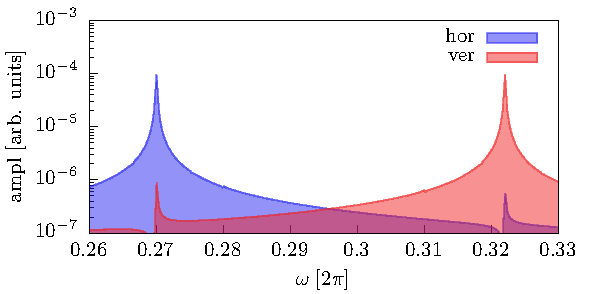
\includegraphics[width=0.7\linewidth]{figures/spectrum_plot}
    \caption{
        This example plot shows the fourier transform of horizontal and vertical particle motion
        from simulations with an AC-dipole and coupling sources. The vertical and horizontal fractional 
        driven tunes are $Q_x^d=0.270$ and $Q_y^d=0.322$.
    }
    \label{fig_cplx_spctr}
\end{figure}
Figure~\ref{fig_cplx_spctr} shows the spectrum of $h_x^+$ and $h_y^+$ excited by an AC-dipole and with coupling.
The driven fractional tunes are $Q_x^d=0.270$, $Q_y^d=0.322$. The respective main lines are well dominating the spectrum
and the secondary lines induced by coupling are clearly visible at the position of the respective other plane's tune.
With this one can introduce a shorthand notation for the spectral lines $\four{h_z^\pm}(n_xQ_x+n_yQ_y)$:
%
\begin{align}
    H^\pm(n_x,n_y) &= \four{h_x^\pm}(n_xQ_x+n_yQ_y) \notag\\
    V^\pm(n_x,n_y) &= \four{h_y^\pm}(n_xQ_x+n_yQ_y) 
    \fstop
\end{align}
%
If the BPM calibration is not perfect the measured $H$ and $V$ lines are not proportional w.r.t. each other:
\newcommand{\meas}{^\text{meas}}
%
\begin{align}
   x\meas &= C_x x \notag \\ 
   y\meas &= C_y y
   \fstop
\end{align}
%
The calibration factors $C_{x/y}$ cancel out if one devides the spectral line by the amplitude of
the main line:
%
\begin{align}
    A_{0,n_y} &= \frac{H^+(0,n_y)}{\left|H^+(1,0)\right|} \notag \\
    B_{n_x,0} &= \frac{V^+(n_x,0)}{\left|V^+(0,1)\right|} 
    \fstop
\end{align}
%
Important for the coupling calculation are the following normalised spectral lines:
%
\begin{align}
    A_{0,1}&=\frac{H^+(0,1)}{\left|H^+(1,0)\right|}
      &= 2i\sqrt{\frac{J_y}{J_x}}\conj{f_{1001}} \e{-i\varphi_{y}}
    \label{eq_A01} \\
    B_{1,0}&=\frac{V^+(1,0)}{\left|V^+(0,1)\right|}
      &= 2i\sqrt{\frac{J_x}{J_y}}{f_{1001}} \e{-i\varphi_{x}}
    \label{eq_B10}
\end{align}
which contain $f_{1001}$ and
\begin{align}
    A_{0,-1}&=\frac{H^+(0,-1)}{\left|H^+(1,0)\right|}
      &= 2i\sqrt{\frac{J_y}{J_x}}\conj{f_{1010}} \e{i\varphi_{y}}
    \label{eq_A0-1} \\
    B_{-1,0}&=\frac{V^+(-1,0)}{\left|V^+(0,1)\right|}
      &= 2i\sqrt{\frac{J_x}{J_y}}\conj{f_{1010}} \e{i\varphi_{x}}
    \label{eq_B-10}
\end{align}
%
which contain $f_{1010}$.

The coupling RDTs $f_{1010}$ and $f_{1001}$ can then be calculated by combining Eqs~(\ref{eq_A01}) with (\ref{eq_B10})
and Eqs~(\ref{eq_A0-1}) with (\ref{eq_B-10}), respectively:
%
\begin{align}
    \left|f_{1001}\right| &= \frac{1}{2}\sqrt{\left| A_{0,1}B_{1,0} \right|} \notag \\
    \left|f_{1010}\right| &= \frac{1}{2}\sqrt{\left| A_{0,-1}B_{-1,0} \right|}
    \label{eq_abs_f_from_AB}
    \fstop
\end{align}
%
The normalised spectral lines $A_{0,n_y}$ and $B_{n_x,0}$ are the Fourier components of the complex
coordinates. But only the projections onto the real axis can be measured. The next step is to calculate
the complex coordinates from the measured ones.

Since $h_z^\pm = z \pm ip_z$ the complex coordinate can be obtained from positon and momentum.
BPMs can only measure position but using the position data from a second BPM one can reconstruct the momentum.
The propagation of complex C-S coordinates through a region that is empty of nonlilnearities reads
%
\begin{equation}
    \begin{pmatrix}
        z\\p_z
    \end{pmatrix}_b = \mat{R}_{ab} 
    \begin{pmatrix}
        z\\p_z
    \end{pmatrix}_a
\end{equation}
%
where the transfer matrix $\mat{R}_{ab}$ is a simple rotation matrix as discussed in section~\ref{sec_intro_cs}.
From this one can reconstruct the momentum:
%
\begin{equation}
    p_a = \frac{x_b}{\cos\Delta} + x_a \tan\Delta
\end{equation}
%
where $\Delta$ is the deviation from $\pi/2$ of the phase advance between the two positions $s_a$ and $s_b$.
Therefore:
%
\begin{equation}
    h_z^\pm(s_a) = z_a - i \left(\frac{z_b}{\cos\Delta} + z_a\tan\Delta \right) = z_a(1-i\tan\Delta) - i \frac{z_b}{\cos\Delta}
    \fstop
\end{equation}
%
Since the Fourier transform is linear, this identity can be propagated to the spectral lines:
%
\begin{equation}
    H^+(n_x,n_y)_a = (1-i\tan\Delta)H(n_x,n_y)_a - \frac{i}{\cos\Delta}H(n_x,n_y)_b
    \label{eq_reconstr_cplx}
\end{equation}
where $H(n_x,n_y)$ is the measured spectral line which is just the real projection of the complex line. 
%
Under the assumption that the region between $s_a$ and $s_b$ is free from non-linearities and coupling
the action $J_z$ does not change between the two positions and
%
\begin{align}
    |H(1,0)_a| &= |H(1,0)_b| = \sqrt{2J_x} \notag\\
    |V(0,1)_a| &= |V(0,1)_b| = \sqrt{2J_y}
    \fstop
\end{align}
%
This allows to express the real normalised spectral lines as
%
\begin{align}
    A(0,n_y)_a &= \frac{H(0,n_y)_a}{\left| H(1,0)_a \right|} = \frac{H(0,n_y)_a}{\left| H(1,0)_b \right|} \notag \\
    B(n_x,0)_a &= \frac{V(n_x,0)_a}{\left| V(0,1)_a \right|} = \frac{V(n_x,0)_a}{\left| V(0,1)_b \right|} 
    \fstop
\end{align}
%
This can be plugged into the reconstruction formula \eqref{eq_reconstr_cplx}
%
\begin{equation}
    \frac{H^+(n_x,n_y)_a}{H(1,0)_i} = (1-i\tan\Delta)A(n_x,n_y)_a - \frac{i}{\cos\Delta}A(n_x,n_y)_b
    \label{eq_reconstr_from_norm}
\end{equation}
%
Together with the identity
%
\begin{equation}
    H(1,0) = \frac{1}{2} \left( H^+(1,0) + {H^-(1,0)}\right) = \frac{1}{2}H^+(1,0)
\end{equation}
%
because $H^-(1,0) = 0$, one can express $A^+(0,n_y)$ and $B(n_x, 0)$ in terms of normalised real spectral lines
%
\begin{align}
    2A^+(n_x,n_y)_a = (1-i\tan\Delta)A(n_x,n_y)_a - \frac{i}{\cos\Delta}A(n_x,n_y)_b \notag \\
    2B^+(n_x,n_y)_a = (1-i\tan\Delta)B(n_x,n_y)_a - \frac{i}{\cos\Delta}B(n_x,n_y)_b
    \label{eq_recon_AB}
\end{align}
%

Which can now be plugged in Eq~(\ref{eq_f0101_f0110}) to calculate the amplitude of the coupling RDTs
$f_{1001}$ and $f_{1010}$. To get the phase the starting point is, again, Eqs~(\ref{eq_A01}) -- (\ref{eq_B-10}).
The phases of $A_{0.1},\,B_{1,0},\,A_{0,-1},\,B_{-1,0}$ contain the phases of the RDTs:
%
\begin{align}
  \text{arg}(A_{0,1}) &= -q_{1001} -\varphi_y +\tfrac{\pi}{2} \\
  \text{arg}(B_{1,0}) &= q_{1001} -\varphi_x +\tfrac{\pi}{2} \\
  \text{arg}(A_{0,-1}) &= -q_{1010} +\varphi_y +\tfrac{\pi}{2} \\
  \text{arg}(B_{-1,0}) &= -q_{1010} +\varphi_x +\tfrac{\pi}{2}
  \label{eq_argA10B01}
\end{align}
%
where the phase $\frac{\pi}{2}$ comes from the factor $i$ and the phases of the RDTs are defined as
%
\begin{align}
  q_{1001} &\equiv \text{arg}(f_{1001})\\
  q_{1010} &\equiv \text{arg}(f_{1010})
  \fstop
  \label{eq_arg_f1001}
\end{align}
%
From \eqref{eq_argA10B01} one gets two expressions for each RDT phase:
%
\begin{equation}
  \begin{matrix*}[l]
  q_{1001} &= -\arg{A_{0,1}}-\varphi_y + \tfrac{\pi}{2} &= \arg{B_{1,0}}+\varphi_x -\tfrac{\pi}{2}\\
  q_{1010} &= -\arg{A_{0,-1}} +\varphi_y + \tfrac{\pi}{2} &= -\arg{B_{-1,0}}+\varphi_x +\tfrac{\pi}{2}
  \label{eq_q1001q1010}
  \end{matrix*}
\end{equation}
%
which can finally be used to calculate the RDTs using \eqref{eq_abs_f_from_AB}.

% --------------------------------------------------------------------------------------------------
% --------------------------------------------------------------------------------------------------
% Forced motion
% --------------------------------------------------------------------------------------------------
\section{Forced motion}

This section will introduce the process of optics measurements with an AC-dipole. As stated above,
the effect of the driving of the beam motion has to be compensated and the foundation for this
compensation will be explained in the following subsections.

% --------------------------------------------------------------------------------------------------
% Linear motion with AC dipole
% --------------------------------------------------------------------------------------------------
\subsection{Linear motion with AC dipole}
\newcommand{\Qd}[1]{Q^{d}_{#1}}
\label{sec_driven_coords}

In this section the C-S coordinates of the driven linear motion will be derived \cite{Miyamoto2010,Peggs1998}. These forced coordinates
can be used to calculate the effect of the AC dipole on linear optics parameters like betatron phase, 
$\beta$~function and linear transverse coupling.

At each turn an AC dipole located at position $s_d$ inflicts a kick to the beam. This kick can be
described in Courant-Snyder coordinates as
%
\begin{equation}
    \Delta h_z(N) = i A_\theta\beta(s_d) \cos(2\pi \Qd{z} N)
\end{equation}
%
depending on the AC dipole frequency $\Qd{z}$ and the turn number $N$. Figure~\ref{fig_ac_kick} shows
a schematic of the beam deflection for several turns.
%
\begin{figure}[h]
    \centering
    \includestandalone{figACkick}
    \caption{
        Schematic of an AC-dipole kick. The deflection $\Delta p_z = A_\theta\beta(s_d)\cos(2\pi i Q_z N)$
        changes with turn number $N$.}
    \label{fig_ac_kick}
\end{figure}
%
For a small $\epsilon$ the C-S coordinates of the beam directly after the AC-dipole reads
%
\begin{equation}
    h_z(s_d + \epsilon, N=0) = h_z(s_d+\epsilon) + \Delta h_z(N=0)
    \label{eq_ackick}
\end{equation}
%
in the first turn where the AC dipole is active. This turn will be denoted with $N=0$.

Under the assumption that the kick strength of the AC-dipole is ramped up slowly enough, this is an
adiabatic process and the effect of the kicks can be added repeatedly for each turn.

Then the coordinates can be propagated to an arbitrary position $s$ in the ring to get the following
expressions:
%
\begin{align}
    h_z(s<s_d, N) &= R_{s-s_d}\left[R^N h_z(s_d) + R^N\Delta h_z(0) + \ldots + R\Delta h_z(N-1)\right] \notag\\
    h_z(s>s_d, N) &= R_{s-s_d}\left[R^N h_z(s_d) + R^N\Delta h_z(0) + \ldots + R\Delta h_z(N-1) + \Delta h_z(N)\right] 
    \komma\\
    h_z(s<s_d, N) &= R_{s-s_d}\left[R^N h_z(s_d) + \sum\limits_{T=1}^N R^T\Delta h_z(N-T)\right] \notag\\
    h_z(s>s_d, N) &= R_{s-s_d}\left[R^N h_z(s_d) + \sum\limits_{T=0}^N R^T\Delta h_z(N-T)\right]
    \komma
    \label{eq_hz_ackick}
\end{align}
%
with $R$ being the rotation map of the linear motion. For simplicity, the following definition has been used:
%
\begin{align}
    &R_{s-s_d} \equiv R(\varphi(s) - \varphi(s_d))\\
    \Rightarrow &R_{s-s_d} h_x = h_x \e{-i\varphi_{s_d s}}
    \fstop
\end{align}
%
The cosine in \eqref{eq_ackick} can be expressed in complex form
%
\begin{align}
    \Delta h_z(N) &= \frac{iA_\theta\beta(s_d)}{2} \left(
        \e{2\pi i \Qd{z} N} +
        \e{-2\pi i \Qd{z} N}
    \right) \notag\\
    &= \frac{iA_\theta\beta(s_d)}{2} \left(
        \delta_+^N + \delta_-^N
    \right)
    \fstop
\end{align}
%
For the second line, $\delta_\pm$ is defined as
%
\begin{equation}
    \delta_\pm = \e{\pm 2\pi i \Qd{z}}
    \fstop
\end{equation}
%
Using the complex form of the cosine, the kick in \eqref{eq_hz_ackick} can be split into left and right moving parts:
%
\begin{multline}
    h_z(s>s_d, N) = \\
    R_{s-s_d}\left[
        R^N h_z(s_d) +
        \frac{iA_\theta\beta(s_d)}{2}\left\{
            \sum\limits_{T=0}^N R^T \delta_+^{N-T}
            + \sum\limits_{T=0}^N R^T \delta_-^{N-T}
        \right\}
        \right]
    \fstop
\end{multline}
%
For the next simplification it shall be noted that
%
\begin{equation}
    \sum\limits_{i=0}^n x^i = \sum\limits_{i=n}^0 x^i = \sum\limits_{j=0}^{n} x^{n-j}
    \fstop
\end{equation}
%
The first transformation is a simple exchange in summation limits. The second one arises from the
change $i\rightarrow j=N-i$ and, thus, $j_0 = N-i_0 = 0$ and $j_1 = N - i_1 = 0$.
Using this, the sums can be brought into the form of a geometric series
%
\begin{align}
    \sum\limits_{T=0}^N R^T\delta_\pm^{N-T}
    &= \sum\limits_{T=0}^N R^{N-T}\delta_\pm^{T} \notag \\
    &=  R ^N \sum\limits_{T=0}^N \left( R^{-1}\delta_\pm \right)^{T} \notag \\
    &=  R ^N \frac{1- (R^{-1}\delta_\pm)^{N+1}}{1 - R^{-1}\delta_\pm}
    \komma
\end{align}
%
and
%
\begin{align}
    \sum\limits_{T=1}^N R^T\delta_\pm^{N-T}
    &= R^N \frac{1- (R^{-1}\delta_\pm)^{N}}{1 - R^{-1}\delta_\pm}
    \fstop
\end{align}
%
The two cases of \eqref{eq_ackick} differ only in one additional exponent of $R^{-1}\delta_\pm$.
\equationref{eq_ackick} can be written as
%
\begin{align}
    h_z(s, N) = R_{s-s_d}R^N 
    \Bigg[&h_z(s_d)  \notag \\
        &+ \frac{iA_\theta\beta(s_d)}{2}\frac{1-(R^{-1}\delta_+)^{N+\Theta(s,s_d)}}{1-R^{-1}\delta_+}  \notag \\
        &+ \frac{iA_\theta\beta(s_d)}{2}\frac{1-(R^{-1}\delta_-)^{N+\Theta(s,s_d)}}{1-R^{-1}\delta_-}
    \Bigg]
    \fstop
\end{align}
%
Furthermore, the terms $R\delta_\pm$ can be written out:
%
\begin{equation}
    R^{-1}\delta_\pm = \e{2\pi i (Q_z \pm \Qd{z})} = \e{\pm 2\pi i Q_z^\pm}
    \komma
\end{equation}
%
and
%
\begin{equation}
    1 - \e{2i\alpha} = -\e{i\alpha}\tfrac{1}{2i} \sin\alpha
    \fstop
\end{equation}
%
Those identities can be used to simplify the exponentials
%
\begin{align}
    h_z(s, N) = R_{s-s_d}R^N 
    \Bigg[&h_z(s_d)  \notag \\
        &+ \frac{A_\theta\beta(s_d)}{4}\frac{1-\e{2\pi i Q_z^+(N+\Theta(s,s_d))}}{\e{i\pi Q_z^+}\sin\left( \pi Q_z^+ \right)}  \notag \\
        &- \frac{A_\theta\beta(s_d)}{4}\frac{1-\e{-2\pi i Q_z^-(N+\Theta(s,s_d))}}{\e{i\pi Q_z^-}\sin\left( \pi Q_z^- \right)}
    \Bigg]
    \fstop
    \label{eq_delta_written_out}
\end{align}
%
The constant part of \eqref{eq_delta_written_out} can be put into 
%
\begin{equation}
    \tilde{h}_z(s_d) \equiv h_z(s_d) + 
    \left(
    \frac{A_\theta\beta(s_d)}{4\sin\left( \pi Q_z^-\right)}\lambda_z \e{i \pi Q_z^-}
    -\frac{A_\theta\beta(s_d)}{4\sin\left( \pi Q_z^+\right)} \e{-i\pi Q_z^+}
    \right)
    \fstop
\end{equation}
%
Now, the driven motion is seperated off:
%
\begin{align}
    h_z(s, N) = R_{s-s_d}R^N 
    \Bigg[&\tilde{h}_z(s_d) 
    \notag \\
        &+ \frac{A_\theta\beta(s_d)}{4\sin\left( \pi Q_z^-\right)} \e{-\pi i Q_z^-(2N+2\Theta(s,s_d)-1)} 
         \notag \\
        &- \frac{A_\theta\beta(s_d)}{4\sin\left( \pi Q_z^+\right)} \e{\pi i Q_z^+(2N+2\Theta(s,s_d) -1)}
    \Bigg]
    \fstop
    \label{eq_driven_simpl}
\end{align}
%
and the linear rotation can be integrated into the terms:
%
\begin{align}
    h_z(s, N) =
        &\tilde{h}_z(s, N) \notag \\
        &+\frac{A_\theta\beta(s_d)}{4\sin\left( \pi Q_z^-\right)}
        \e{i\left[-2\pi NQ_{z} - \varphi_{s_ds} + \pi Q_z^-(2N+2\Theta(s,s_d)-1)\right]}
        \notag\\
        &-\frac{A_\theta\beta(s_d)}{4\sin\left( \pi Q_z^+\right)}
        \e{i\left[2\pi NQ_{z} - \varphi_{s_ds}- \pi Q_z^+(2N + 2\Theta(s,s_d) -1)\right]}
    \fstop
    \label{eq_driven_simpl}
\end{align}
%
Noting that
%
\begin{equation}
  2\Theta(a) - 1 = \text{sgn}(a) \text{, if } a \neq 0
    \komma
\end{equation}
%
\eqref{eq_driven_simpl} can be further simplified\footnote{
    strictly speaking \eqref{eq_driven_simpl2} is valid only for $s\neq s_d$ and one should carefully exclude this case
    in the following. But since a measurement at the exact position of the AC Dipole is not possible in the first place
    this fine detail will be ignored in this work.
    }:
%
\begin{align}
    h_z(s, N) =
        &\tilde{h}_z(s, N) \notag \\
        &+ \frac{A_\theta\beta(s_d)}{4\sin\left( \pi Q_z^-\right)}
        \e{i\left[-2N\pi \Qd{z} - \varphi_{s_ds} + \pi Q_z^-\text{sgn}(s-s_d)\right]} 
        \notag \\
        &- \frac{A_\theta\beta(s_d)}{4\sin\left( \pi Q_z^+\right)}
        \e{i\left[2N\pi \Qd{z} - \varphi_{s_ds} - \pi Q_z^+\text{sgn}(s-s_d)\right]} 
    \fstop
    \label{eq_driven_simpl2}
\end{align}
%
The free motion of the beam is perturbed by two driving modes corresponding to the sum and difference
of natural tune and driven tune. In most applications the ac-dipole strength much greater than the free 
oscillation amplitude $A_\theta\beta(s_d) \gg |\bar{h}_z(s,N)|$.

All derivations in this section have been made for $h_z^+$. It shall be noted here that the negatively turning
coordinate $h_z^-$ has the form
%
\begin{align}
    h_z^-(s, N) =
        &\tilde{h}_z^-(s, N) \notag \\
        &+ \frac{A_\theta\beta(s_d)}{4\sin\left( \pi Q_z^-\right)}
        \e{i\left[2N\pi \Qd{z} + \varphi_{s_ds} - \pi Q_z^-\text{sgn}(s-s_d)\right]} 
        \notag \\
        &- \frac{A_\theta\beta(s_d)}{4\sin\left( \pi Q_z^+\right)}
        \e{i\left[-2N\pi \Qd{z} + \varphi_{s_ds} + \pi Q_z^+\text{sgn}(s-s_d)\right]} 
    \fstop
    \label{eq_driven_simpl2_minus}
\end{align}
%
Subtracting the closed driven closed orbit $\tilde{h}_z$ and with the definition
%
\begin{equation}
    \lambda_z = \frac{\sin(\pi Q_z^-)}{\sin(\pi Q_z^+)}
    \komma
\end{equation}
%
the driven motion can be rewritten in the from
%
\begin{align}
    h_z^\pm(s,N) = 
        \frac{A_\theta}{4\sin\left( \pi Q_z^-\right)}
        \Bigg[ 
            &\e{\pm i\left[-2N\pi \Qd{z} - \varphi_{s_ds} + \pi Q_z^-\text{sgn}(s-s_d)\right]} 
            \notag \\
            &- \lambda_z
             \e{\pm i\left[2N\pi \Qd{z} - \varphi_{s_ds} - \pi Q_z^+\text{sgn}(s-s_d)\right]} 
        \Bigg]
    \komma
    \label{eq_driven_hz_final}
\end{align}
%
which is used in other works \cite{Miyamoto2008, Miyamoto2010}. 


\subsection{Compensation of linear parameters}

This section briefly summarises the compensation of the driven motion for the optics parameters
$\beta$, $\alpha$ and $\phi$ \footnote{\cite{Miyamoto2008} and Ryoichi Miyamoto, private communication, Feb. 2017}.

In an actual measurement the phase and amplitude are calculated from the fourier analysis of the
real signal.
%
\begin{align}
   H(1,0)^\text{free} &= \frac{1}{2}\left( H^+(1,0)^\text{free} + H^-(1,0)^\text{free} \right)\notag \\
   &= \sqrt{2 J_z\beta} \left[ \e{-i\varphi(s) } + \e{i\varphi(s)} \right]
   \label{eq_four_real_free}
\end{align}
%
for the free motion and
%
\begin{align}
   H(1,0)
   % &= \notag \\
   &= \frac{A_\theta}{4\sin(\pi Q_z^-)}\left[
        \e{i\left[-\varphi_{s_ds} + \pi Q_z^-\text{sgn}(s_ds)\right]}
        -\lambda \e{i\left[\varphi_{s_ds} + \pi Q_z^+\text{sgn}(s_ds)\right]}
       \right]
       \label{eq_four_real_driven}
\end{align}
for the driven motion.
%
For the next steps the following trigonometric reformulation is needed:
%
\begin{equation}
  \e{i\left( \alpha + \beta \right)} - \lambda \e{i\left( \alpha - \beta \right)}
  = \e{i\alpha} \left(\e{i\beta} - \lambda\e{-i\beta}\right)
  \fstop
  \label{eq_e_alpha_lambda}
\end{equation}
%
The sum of two oscillations with the same frequency forms a single oscillation, so the $\beta$~term can
be rewritten as
%
\begin{equation}
  B = |B|\e{i\psi}
\end{equation}
with
%
\begin{align}
  |B|^2 &=  \left( \e{i\beta}-\lambda\e{-i\beta} \right)\left( \e{-i\beta} - \lambda\e{i\beta} \right)
  = 1+\lambda^2-2\lambda\cos{2\beta} \notag \\
  \psi&= \atan \frac{\im{B}}{\re{B}} = \atan\left(\frac{1+\lambda}{1-\lambda}\tan \beta\right)
  \fstop
\end{align}
%
Now \eqref{eq_four_real_driven} can be put in this form by defining
%
\begin{align}
  \alpha &\equiv \pi\Qd{z} \text{sgn}(s-s_d) \notag \\
  \beta &\equiv \pi Q_z\text{sgn}(s-s_d) - \varphi_{s_ds}
\end{align}
%
This allows for $H(1,0)$ to be rewritten
%
\begin{align}
  H(1,0) =&\: \frac{A_\theta\beta(s_d)}{4\sin(\pi Q_z^-)}
  \sqrt{1+\lambda^2-2\lambda\cos\left[2\varphi_{s_ds} - \pi Q_z\text{sgn}(s-s_d)\right]} \notag \\
  &\times\e{i\left[ \pi \Qd{z}\text{sgn}(s-s_d) + \psi \right]}
  \fstop
\end{align}
%
Comparing to the free case, \eqref{eq_four_real_free}, the driven phase is defined as 
%
\begin{align}
  \varphi^d_{s_ds} &=  \Qd{z}\text{sgn}(s-s_d) + \psi\notag\\
  &=  \Qd{z}\text{sgn}(s-s_d)
  + \atan\left( \frac{1+\lambda}{1-\lambda}\tan\left( \varphi_{s_ds}-\pi Q_z\text{sgn}(s-s_d)\right) \right)
\end{align}
%
which fullfils the symmetric property
%
\begin{equation}
  (1-\lambda)\tan\left( \varphi^d_{s_ds} -\pi \Qd{z}\text{sgn}(s-s_d) \right)
  =
  (1+\lambda)\tan\left( \varphi_{s_ds} -\pi Q_z\text{sgn}(s-s_d) \right)
  \label{eq_drv_phase_sym}
\end{equation}
%
In order to get the driven Twiss parameters $\alpha^d$, $\beta^d$ and $\gamma^d$, the same relation
between them and the driven phase $\varphi^d$ is imposed:
\begin{equation}
  \frac{\der \varphi^d}{\der s} = \frac{1}{\beta^d}
\end{equation}
%
Taking the derivative of  \eqref{eq_drv_phase_sym} w.r.t. $s$ yields
%
\begin{equation}
  \frac{(1-\lambda)\varphi'^d(s)}{\cos^2\left[ \varphi^d(s) - \pi\Qd{z}\text{sgn}(s-s_d) \right]}
  =
  \frac{(1+\lambda)\varphi'(s)}{\cos^2\left[ \varphi(s) - \pi Q_z\text{sgn}(s-s_d) \right]}
  \komma
\end{equation}
%
where it is assumed that all phases are w.r.t. the position of the AC-dipole $s_d$ and $f'(x)$ denotes
the derivative of the function $f$ with respect to $x$.
Respectively, taking its square yields
\begin{equation}
  \frac{(1-\lambda)}{\cos^2\left[ \varphi^d(s) - \pi\Qd{z}\text{sgn}(s-s_d) \right]} +2\lambda
  =
  \frac{(1+\lambda)^2}{\cos^2\left[ \varphi(s) - \pi Q_z\text{sgn}(s-s_d) \right]} -2\lambda
  \fstop
  \label{<+label+>}
\end{equation}
%
Both equations can be used to cancel $\cos\left[ \varphi^d(s) - \pi \Qd{z}\text{sgn}(s-s_d) \right]$:
%
\begin{equation}
  \frac{1}{\varphi'^d(s)} = 
  \frac{1+\lambda^2-2\lambda\cos\left[ 2\varphi(s) - 2\pi Q_z\text{sgn}(s-s_d)\right]}{1-\lambda^2}
  \frac{1}{\varphi'(s)}
\end{equation}
%
which, finally, is the formula to compute the driven $\beta$~function:
%
\begin{equation}
  \beta^d(s) =
  \frac{1+\lambda^2-2\lambda\cos\left[ 2\varphi(s) - 2\pi Q_z\text{sgn}(s-s_d)\right]}{1-\lambda^2}
  \beta(s)
\end{equation}
%
The driven $\alpha$ function follows from the definition of the free $\alpha$~function:
\begin{align}
  \alpha^d(s) &=  \frac{1}{2}\frac{\der \beta^d}{\der s}\notag \\
  &= 
  \frac{1+\lambda^2-2\lambda\cos\left[ 2\varphi(s) - 2\pi Q_z\text{sgn}(s-s_d)\right]}{1-\lambda^2}
  \alpha(s) \notag \\
  &\quad- 2\lambda \sin\left[ 2\varphi(s) - 2\pi Q_z\text{sgn}(s-s_d) \right]
  \label{eq_drv_alpha}
\end{align}
%
Comparing the amplitude of the driven motion \eqref{eq_z_drv} with the form \eqref{eq_drv_x_from_h_tpl}
the driven action $J_x^d$ can be deduced:
%
\begin{align}
  \sqrt{2J_z^d\beta_z^d(s)} &= 
  \frac{A_\theta\sqrt{\beta(s_d)\beta(s)}}{4\sin(\pi Q_z^-)}
  \sqrt{1+\lambda^2-2\lambda\cos\left[2\varphi_{s_ds} - \pi Q_z\text{sgn}(s-s_d)\right]} \notag \\
  \Rightarrow J_z^d &=  \frac{A_\theta^2\beta(s_d)(1-\lambda^2)}{32 \sin^2(\pi Q_z^-)}
  \fstop
  \label{eq_drv_Jy}
\end{align}
%
The expressions for the driven optics parameters $\beta^d$, $\alpha^d$, $\varphi^d$ and $J^d$ derived
in this section can be used to compensate the effect of the driven motion on the measurement and enable
an easy measurement leveraging the advantages of an AC-dipole for optics measurements in circular
accelerators.
